\documentclass[english,man]{apa6}

\usepackage{amssymb,amsmath}
\usepackage{ifxetex,ifluatex}
\usepackage{fixltx2e} % provides \textsubscript
\ifnum 0\ifxetex 1\fi\ifluatex 1\fi=0 % if pdftex
  \usepackage[T1]{fontenc}
  \usepackage[utf8]{inputenc}
\else % if luatex or xelatex
  \ifxetex
    \usepackage{mathspec}
    \usepackage{xltxtra,xunicode}
  \else
    \usepackage{fontspec}
  \fi
  \defaultfontfeatures{Mapping=tex-text,Scale=MatchLowercase}
  \newcommand{\euro}{€}
\fi
% use upquote if available, for straight quotes in verbatim environments
\IfFileExists{upquote.sty}{\usepackage{upquote}}{}
% use microtype if available
\IfFileExists{microtype.sty}{\usepackage{microtype}}{}

% Table formatting
\usepackage{longtable, booktabs}
\usepackage{lscape}
% \usepackage[counterclockwise]{rotating}   % Landscape page setup for large tables
\usepackage{multirow}		% Table styling
\usepackage{tabularx}		% Control Column width
\usepackage[flushleft]{threeparttable}	% Allows for three part tables with a specified notes section
\usepackage{threeparttablex}            % Lets threeparttable work with longtable

% Create new environments so endfloat can handle them
% \newenvironment{ltable}
%   {\begin{landscape}\begin{center}\begin{threeparttable}}
%   {\end{threeparttable}\end{center}\end{landscape}}

\newenvironment{lltable}
  {\begin{landscape}\begin{center}\begin{ThreePartTable}}
  {\end{ThreePartTable}\end{center}\end{landscape}}

  \usepackage{ifthen} % Only add declarations when endfloat package is loaded
  \ifthenelse{\equal{\string man}{\string man}}{%
   \DeclareDelayedFloatFlavor{ThreePartTable}{table} % Make endfloat play with longtable
   % \DeclareDelayedFloatFlavor{ltable}{table} % Make endfloat play with lscape
   \DeclareDelayedFloatFlavor{lltable}{table} % Make endfloat play with lscape & longtable
  }{}%



% The following enables adjusting longtable caption width to table width
% Solution found at http://golatex.de/longtable-mit-caption-so-breit-wie-die-tabelle-t15767.html
\makeatletter
\newcommand\LastLTentrywidth{1em}
\newlength\longtablewidth
\setlength{\longtablewidth}{1in}
\newcommand\getlongtablewidth{%
 \begingroup
  \ifcsname LT@\roman{LT@tables}\endcsname
  \global\longtablewidth=0pt
  \renewcommand\LT@entry[2]{\global\advance\longtablewidth by ##2\relax\gdef\LastLTentrywidth{##2}}%
  \@nameuse{LT@\roman{LT@tables}}%
  \fi
\endgroup}


  \usepackage{graphicx}
  \makeatletter
  \def\maxwidth{\ifdim\Gin@nat@width>\linewidth\linewidth\else\Gin@nat@width\fi}
  \def\maxheight{\ifdim\Gin@nat@height>\textheight\textheight\else\Gin@nat@height\fi}
  \makeatother
  % Scale images if necessary, so that they will not overflow the page
  % margins by default, and it is still possible to overwrite the defaults
  % using explicit options in \includegraphics[width, height, ...]{}
  \setkeys{Gin}{width=\maxwidth,height=\maxheight,keepaspectratio}
\ifxetex
  \usepackage[setpagesize=false, % page size defined by xetex
              unicode=false, % unicode breaks when used with xetex
              xetex]{hyperref}
\else
  \usepackage[unicode=true]{hyperref}
\fi
\hypersetup{breaklinks=true,
            pdfauthor={},
            pdftitle={Applying Network Analysis to Ideal Point Personality Item Responses},
            colorlinks=true,
            citecolor=blue,
            urlcolor=blue,
            linkcolor=black,
            pdfborder={0 0 0}}
\urlstyle{same}  % don't use monospace font for urls

\setlength{\parindent}{0pt}
%\setlength{\parskip}{0pt plus 0pt minus 0pt}

\setlength{\emergencystretch}{3em}  % prevent overfull lines

\ifxetex
  \usepackage{polyglossia}
  \setmainlanguage{}
\else
  \usepackage[english]{babel}
\fi

% Manuscript styling
\captionsetup{font=singlespacing,justification=justified}
\usepackage{csquotes}
\usepackage{upgreek}

 % Line numbering
  \usepackage{lineno}
  \linenumbers


\usepackage{tikz} % Variable definition to generate author note

% fix for \tightlist problem in pandoc 1.14
\providecommand{\tightlist}{%
  \setlength{\itemsep}{0pt}\setlength{\parskip}{0pt}}

% Essential manuscript parts
  \title{Applying Network Analysis to Ideal Point Personality Item Responses}

  \shorttitle{An Exploratory Analysis}


  \author{Dan Simonet\textsuperscript{1}~\& Christopher M. Castille\textsuperscript{2}}

  \def\affdep{{"", ""}}%
  \def\affcity{{"", ""}}%

  \affiliation{
    \vspace{0.5cm}
          \textsuperscript{1} Montclair State University\\
          \textsuperscript{2} Nicholls State University  }

  \authornote{
    \newcounter{author}
    Dan Simonet is an Assistant Professor of Psychology at Montclair State
    University. Christopher M. Castille is an Assistant Professor of
    Management and Marketing at Nicholls State University.

                      Correspondence concerning this article should be addressed to Dan Simonet, Postal address. E-mail: \href{mailto:my@email.com}{\nolinkurl{my@email.com}}
                          }


  \abstract{Personality researchers have recently taken interest in two
methodological innovations network analysis and ideal point item writing
strategies. The former suggests that personality is best understood as a
system of mutually reinforcing actions while the latter allows more
precise measurement of personality components. Here, we explore the
value of integrating these two innovations by exploring the network
properties of a Big Five inventory constructed with ideal-point items.}
  \keywords{ideal point, personality, network analysis \\

    \indent Word count: XXXX
  }





\usepackage{amsthm}
\newtheorem{theorem}{Theorem}
\newtheorem{lemma}{Lemma}
\theoremstyle{definition}
\newtheorem{definition}{Definition}
\newtheorem{corollary}{Corollary}
\newtheorem{proposition}{Proposition}
\theoremstyle{definition}
\newtheorem{example}{Example}
\theoremstyle{remark}
\newtheorem*{remark}{Remark}
\begin{document}

\maketitle

\setcounter{secnumdepth}{0}



\section{\texorpdfstring{\textbf{Introduction}}{Introduction}}\label{introduction}

Recent findings suggests self-report inventories conform to an ideal
point process in which persons endorse items only to the extent the item
content reflects the respondent's level of the attribute, or \(\Theta\).
Modeling the correct response process in personality assessment produces
several psychometric benefits, such as improved dimensionality, higher
total test information, and revelation of curvilinear effects (Drasgow,
Chernyshenko, \& Stark, 2010). One reason for such gains is the ideal
point perspective retains items assessing low, intermediate, and high
trait values and, thus, creates an instrument providing greater
measurement precisions across a broad range of a targeted attribute.

Due to its methodological nature, ideal-point research has focused
largely on technical issues, such as appropriate item writing
strategies, model fitting, or validity gains. Surprisingly little work
has been done to explore the advantages of ideal-point inventories to
understanding personality itself, such as explaining where traits come
from, how they operate, and how they produce differences in behavior.
These questions lie at the heart of the discipline (Fleeson \&
Jayawickreme, 2015) and carry theoretical implications for understanding
why personality predicts work behavior and how personality changes over
time (i.e., selection and development). Given that ideal-point
inventories capture a wider array of elemental differences in emotions,
thoughts, and behaviors constituting the Big Five, they may especially
suited to identifying plausible mechanisms through which personality
processes (deliberation, emotional regulation) accrue to form traits
(individual differences).

Drawing upon a psychometric network approach to individual differences
(Cramer et al., 2012), we recast the Big Five as a dynamic system of
directly interacting feelings, thoughts, and behaviors. Rather than
treat \enquote{hidden traits} as causal forces lying behind stable
behavioral patterns, the network approach models traits as consequences
of mutually reinforcing interactions between specific thoughts,
feelings, and behaviors (see Figure 1 for illustration). From this
perspective, discrete actions like working hard to attain long-term
goals, planning one's week, and focusing on a task to completion in a
person high on Conscientiousness do not co-occur because of a top-down
latent disposition, but because deciding to care about a long-term goal
leads one to be more disciplined in allocation of personal resources.
Forces bonding autonomous acts into trait clusters might be shared
biological origins, learning principles, socially enforced norms, or
functional aims that produce accretion of multiple explanatory
mechanisms which unite for causal, homeostatic, or logical reasons
(Cramer et al., 2012; Fleeson \& Jayawickreme, 2015; Wood, Gardner, \&
Harms, 2015).

\begin{figure}

{\centering 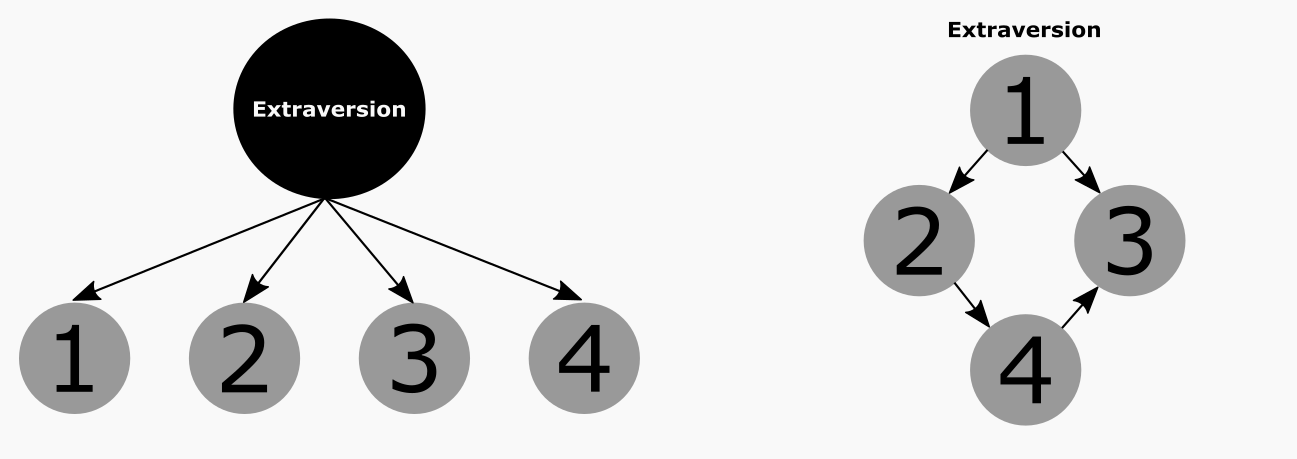
\includegraphics[width=4.32in]{C:/Users/Simmy566/Documents/Ideal-Point-Items-and-Network-Analysis-Project/Latnet_fig1} 

}

\caption{Trait model according to a latent variable (left panel) and a network perspective (right panel)}\label{fig:unnamed-chunk-2}
\end{figure}

More importantly, the network perspective can provide a better view of
the cognitive, motivational, and functional dynamics characterizing the
development of the personality system, therefore favoring empirical
investigations of such mechanisms. Incorporating ideal point items may
offer further insight into trait development by pinpointing intermediate
ranges of a trait continuum (i.e., nodes) which incrementally
\enquote{bridge} personality components across distinct clusters
(Borsboom \& Cramer, 2013). For instance, the conscientiousness item
\enquote{I tend to be disorderly but also like to keep certain things
tidy} may bridge the agreeableness item of \enquote{I don't like to let
others down} to the remaining network of conscientiousness items. Why?
Because development in compassion arising from social roles (e.g.,
serious relationships, care for family) might elevate conscientiousness
by causing individuals to start bringing personal affairs in order. That
is, when we begin caring about others we may try to get our \enquote{act
together} in order to meet social responsibilities. Such effects may be
less evident in extreme items (I always keep my affairs in order)
because developmental processes are gradual and better seen in
intermediate steps. By finding and pulling these functional levers
(i.e., intermediate items), we may be able to nudge people to change in
productive ways on multiple dimensions (or traits) which has
implications for executive coaching and trait interventions.

The current study unifies these methodological innovations by applying
network analyses to a Big Five instrument developed with ideal-point
item writing strategies. We contrast four major network properties with
research exploring similar properties of common Big Five inventories
(Cramer et al., 2012; Constantini et al., 2015; Constantini \& Perugini,
2016). The first is the topology, or \emph{large-scale structure}, of
the Big Five including global node arrangement and degree to which nodes
cluster together while distances between any two nodes remain small
(\emph{small-worldness}; Constantini et al., 2015). Two, we identify the
nature and content of cross-trait item pairings to identify possible
\emph{bridging} components explaining observed covariance between trait
factors (e.g., why do agreeable people tend to be conscientious). Three,
we compare the most \enquote{central} and \enquote{peripheral} nodes
with the nature of the central facets identified in past publications.
Nodes which are central play a more prominent role in connecting
elements of the personality system and, consequentially, may be idea
targets for intervention if desiring to shift one's personality.
Finally, given the general importance of emotional stability and
conscientiousness for job performance across occupations, we examine the
\emph{shortest} pathways that may explain the route through which
changes in emotional stability (conscientiousness) may facilitate
changes in conscientiousness (emotional stability). In all cases, we
highlight areas where ideal-point items play a role in facilitating
information flow in the Big Five network.

\section{\texorpdfstring{\textbf{Methods and
Results}}{Methods and Results}}\label{methods-and-results}

Given space limits yet novelty of network terminology, the methods and
results are presented concurrently.

We report how we determined our sample size, all data exclusions (if
any), all manipulations, and all measures in the study.

\subsection{Participants}\label{participants}

\subsection{Measure}\label{measure}

\subsection{Material}\label{material}

\subsection{Procedure}\label{procedure}

\subsection{Data analysis}\label{data-analysis}

We used R (3.3.1, R Core Team, 2016) and the R-packages \emph{bitops}
(1.0.6, Steve Dutky initial R port, Martin Maechler; revised, \& Steve
Dutky, 2013), \emph{bootnet} (1.0.0, Epskamp, Borsboom, \& Fried, 2017),
\emph{careless} (1.0, Yentes, 2016), \emph{corrr} (0.2.1, Jackson,
2016), \emph{dplyr} (0.5.0, Wickham \& Francois, 2016), \emph{Formula}
(1.2.1, Zeileis \& Croissant, 2010), \emph{ggplot2} (2.2.1, Wickham,
2009), \emph{Hmisc} (4.0.3, Harrell Jr, Charles Dupont, \& others.,
2017), \emph{kableExtra} (0.4.0, Zhu, 2017), \emph{knitr} (1.17, Xie,
2015), \emph{lattice} (0.20.33, Sarkar, 2008), \emph{lavaan}
(0.5.23.1097, Rosseel, 2012), \emph{mgm} (1.2.1, Haslbeck \& Waldorp,
2016), \emph{pander} (0.6.0, Darczi \& Tsegelskyi, 2015), \emph{papaja}
(0.1.0.9492, Aust \& Barth, 2017), \emph{psych} (1.6.12, Revelle, 2016),
\emph{purrr} (0.2.2, Wickham, 2016), \emph{qgraph} (1.4.2, Epskamp,
Cramer, Waldorp, Schmittmann, \& Borsboom, 2012), \emph{RCurl}
(1.95.4.8, Lang \& CRAN team, 2016), \emph{readr} (1.0.0, Wickham,
Hester, \& Francois, 2016), \emph{stringr} (1.2.0, Wickham, 2017a),
\emph{survival} (2.40.1, Terry M. Therneau \& Patricia M. Grambsch,
2000), \emph{tibble} (1.2, Wickham, Francois, \& Mller, 2016),
\emph{tidyr} (0.6.1, Wickham, 2017b), and \emph{tidyverse} (1.1.1,
Wickham, 2017c) for all our analyses.

\subsubsection{Estimating and Visualizing the
Network}\label{estimating-and-visualizing-the-network}

Personality networks present items as nodes connected by edges
representing statistical relationships. We implemented a Gaussian
Graphical Model (GGM) on a polychoric correlation matrix using a
graphical least absolute shrinkage and selection (glasso) with the
extended EBIC criterium in \emph{qgraph} 1.4.3 (Epskamp, Borsboom, \&
Fried, 2017; Friedman et al., 2008). There are two things to note.
First, the glasso avoids spurious associations by using
\emph{regularization} to assign penalties so all edges are shrunk with
small edges being set to zero. This results in a \emph{sparse} (i.e.,
conservative) network that safeguards against overfitting by modeling
covariance among components with as few connections as possible. Second,
because the network uses partial correlations, all edges imply a
relationship exists after controlling for all other nodes. Because the
model is uniquely specified, it facilitates clear and unambiguous
interpretation of edge-weight parameters as the strength of
\emph{unique} associations providing a putative causal skeleton. Given
the larger number of items, the EBIC hyperparameter was set to a
conservative .8 to err on the side of caution and we hide all partial
correlations less than .05 for visual clarity.

The initial network presented in Figure 1 (item labels are provided in
Table 1) has 1,339 nonzero edges out of 11,175 possible edges (12\%)
suggesting a relatively sparse network. Several insights can be inferred
about the general architecture and generating processes of the Big Five.
One, similar to Cramer et al (2012), there is clustering for four of the
Big Five with Openness showing less cohesion. Two, it is possible to
identify \enquote{pockets} of high interactivity (i.e., facets or unique
item effects) by highlighting nodes with numerous, densely connected
edges as well as their pathways to the larger network. For instance,
there is a leadership pocket in the bottom of the extraversion network
consisting of items about taking charge (Ex33), following others (Ex31),
or enjoyment of project leadership (Ex34). Notice this cluster -- while
embedded in extraversion -- is also distinct because it is only
connected to the larger network by a few nodes, such as the belief one
is able to persuade (Ex35) and make friends (Ex15) coupled with efforts
to engage others (Ex5) and being averse to mediocre work (Co16). Its
distinction and peripheral placement may suggest assertive aspects of
Extraversion arise from social skills, effort to meet others, and a
desire to improve the status quo (i.e., not be mediocre). This reasoning
is aligned with a cognitive-affective processing and functional approach
to personality in which abilities, values, and efficacy produce trait
covariation (Wood et al., 2015). Three, items along the Big Five borders
may illuminate unique developmental pathways or feedback loops through
which change spreads between traits. Take the borders between
conscientiousness and openness. The nodes in the lower left suggest the
enjoyment of solving complex problems (O2, O3, O8) is positively linked
to a high drive for achievement (Co17, Co18, Co19) whereas nodes in the
center left show tolerance for variety (O9, O10, O11) as
\emph{negatively} linked to preference for order (Co8, Co7, Co6, Co9).
This suggests countervailing forces such that mutually reinforcing gains
in two Openness components may be associated with diverging effects in a
person's Conscientiousness network (e.g., more industrious but lower
order). Interestingly, there are multiple boundary spanning items with
ideal-point properties (e.g., O9, Es16, Es27, Ex17, Ex18, Co2, Co8,
Co11, Co12, Ag7, Ag14, Ag21) suggesting they help elaborate unique ways
trait networks collide.

\begin{figure}[htbp]
\centering
\includegraphics{Ideal_Point_Items_and_Network_Analysis_files/figure-latex/unnamed-chunk-4-1.pdf}
\caption{\label{fig:unnamed-chunk-4}Network representation of 168
ideal-point inventory modeled after the NEO-PI facet structure. Each
item is represented by a node, and the node number corresponds to the
item statements in Table 1. Nodes are connected by green (red) lines if
they are positively (negatively) correlated. Line thickness corresponds
to correlation strength. The spring-bsaed algorithm (Fruchterman \&
Reingold, 1991) used to generate the graph places strongly correlated
nodes closely together and towards the middle of the graph.}
\end{figure}

The small world index was 2.35, which is higher than the values of 1.01
reported on the HEXACO facets (Constantini et al., 2015) but slightly
lower than the 3 threshold recommended for describing the entire network
as a small-world (Watts \& Strogatz, 1998). As noted by Constantini and
Perugi (2016), a small-world structure may be masked when items conform
to a simple structure. This suggests the current inventory is more
clearly organized into separate sub-systems (e.g., the Big Five with
exception of Openness) which themselves influence one another by means
of bridging connections. When a network shows small-worldness, changes
in any random part of the network could quickly spread across the whole
system (Watts \& Strogatz, 1998).To illustrate the bridging components
linking the larger Big Five network, the initial network was arranged by
the Big Five clusters with only partial correlations \textgreater{} .10
displayed (see Figure 2). Eighteen cross-trait item pairings remained
(presented in Table 2) which might explain the often-substantial
inter-correlations observed between personality factors. Whereas the
reason for some linkages is not apparent (Ag23/Co3), others are commonly
alluded to in the literature such as the demand for both positive affect
and difficult goals in being driven at work (e.g., Co15/Ex22).

\begin{table}[!h]

\caption{\label{tab:unnamed-chunk-5}Eighteen Bridging Item Pairs}
\centering
\resizebox{\linewidth}{!}{\begin{tabular}[t]{lll}
\toprule
ItemLabels & FirstItem & SecondItem\\
\midrule
Ag28.O26 & People often tell me Im a genuine person & People talk to me because I empathize with how they feel\\
Ag13.Co5 & Honesty is the foundation of any good relationship & It is best to be careful when a decision has significant consequence\\
Ag14.Co25 & I feel the urge to confide in others & Although I am capable of motivating myself to complete tasks I prefer to have someone else prompting\\
Ag26.Co11 & Manipulating others can be helpful & I have lied to protect other people\\
Ag23.Co3 & Fine being anonymous when giving money to charity & On occasion it can be helpful to consider all options when making decisions\\
\addlinespace
Co5.O24 & It is best to be careful when a decision has significant consequences & If an emotion is really obvious then I can probably identify it\\
Co10.O9 & I like to plan my days in advance & I prefer stability or consistency to variety and change\\
Co18.O8 & I aspire to do well in more areas compared to most people & I really enjoy trying to tackle the most complex problems imaginable\\
Co3.O24 & On occasion it can be helpful to consider all options when making decisions & If an emotion is really obvious then I can probably identify it\\
Co15.Ex22 & I avoid setting goals but when I do I set extremely easy goals & I generally prefer activities that require little energy\\
\addlinespace
Ex9.Es18 & I always look at the bright side of life & I always feel great about the person that I am\\
Ex16.Es2 & I am always friendly to people & I like to consider myself as a very easygoing person\\
Ex22.O3 & I generally prefer activities that require little energy & I dislike thinking too hard about things\\
Ex12.O20 & I always hide my true feelings from people & I am unable to reciprocate when someone talks about their feelings\\
Co1.Es14 & I find that most all of my decisions are impulsive & I feel most alive when I give into my urges\\
\addlinespace
Co11.Es13 & I have lied to protect other people & Sometimes I do things I later regret\\
Ag25.Ex12 & I always hide my motives to get what I want & I always hide my true feelings from people\\
Ag3.Ex16 & When someone is in need I feel as though I have to help & I am always friendly to people\\
\bottomrule
\end{tabular}}
\end{table}

\begin{figure}[htbp]
\centering
\includegraphics{Ideal_Point_Items_and_Network_Analysis_files/figure-latex/unnamed-chunk-6-1.pdf}
\caption{\label{fig:unnamed-chunk-6}Same network results from Figure 1
rearranged by Big Five groupings and restricted to display partial
correlations .10 or greater. Visualized edges depict strong residual
item associations within and between trait factors.}
\end{figure}

\subsubsection{Centrality Estimation}\label{centrality-estimation}

A typical way of assessing node importance is to compute centrality
indices of the network structure (Costantini et al., 2015; Newman, 2010;
Opsahl, Agneessens, \& Skvoretz, 2010). Three such measures are (1)
\emph{node strength}, quantifying how well a node is directly connected
to other nodes by summing all of its absolute edges, (2)
\emph{closeness}, quantifying how well a node is indirectly connected to
other nodes by taking the inverse of all shortest path lengths between
the node and all other nodes, and (3) \emph{betweeness}, quantifying how
important a node is in the average path between two other nodes. While
such indices often agree, it is possible for a node to be high on one
index but low on another. For instance, the Amsterdam airport would
score high on \emph{strength} as many airports fly planes in and out of
Amsterdam. Comparatively, the airport in Anchorage, Alaska, while low on
strength in terms of absolute number of connections, is actually higher
than Amsterdam on \emph{betweenness} because it serves as a common hub
indirectly connecting many international airports to each other via
oversea flights.

The centrality plots appear in Figure 4. Several Agreeableness and
Conscientiousness items stand out as highly influential, especially
those dealing with manipulation and indifference to others (Ag25, Ag26,
Ag31), deliberation in action and decision making (Co1, Co5, Co20) or
completing the bare minimum to get by (Co31). The items Ex24 (Compared
to extremely energetic people I am somewhat less energetic), Es18 (I
always feel great about the person that I am), Es2 (I like to consider
myself a very easygoing person), and O7 (I enjoy having abstract or
philosophical conversations) had relatively high betweeness-centrality,
meaning they occupied strategic positions connecting several groups of
nodes that would be connected by longer paths without these particular
items. ..Conversely, the items Es26 (Occasionally I panic but usually I
do not), Es20 (On occasion I feel blue but most of the time I don't feel
blue), Ag17 (While I sometimes forgive others to avoid confrontation I
also challenge others), Ex21 (I always take my time even when a faster
pace may be needed), Ex38 (Thought I often look on the bright side of
life I am usually more realistic in my outlook), and O29 (If I were
given two problems to work on, one familiar and the other novel, I'd
spend an equal amount on both.) were low on multiple centrality indices
suggesting they \ldots{}

\begin{figure}[htbp]
\centering
\includegraphics{Ideal_Point_Items_and_Network_Analysis_files/figure-latex/unnamed-chunk-7-1.pdf}
\caption{\label{fig:unnamed-chunk-7}Centrality plot depicting the
betweenness, closeness, and strength of each node.}
\end{figure}

\subsubsection{Shortest Pathway between Emotional Stability and
Conscientiousness}\label{shortest-pathway-between-emotional-stability-and-conscientiousness}

Finally, a network illustrating the shortest paths between all
conscientiousness and emotional stability items was computed (see Figure
5). In comparison to the first network, these networks clarify possible
pathways and mediating items between these two factors. The shortest
path between 2 nodes represents the minimum number of steps needed to go
from one node to another, and is computed using Dijkstra's algorithm
(Dijkstra, 1959). This can be seen as a roadmap including all possible
routes from destination A to destination B, but only one of these routes
being quicker---this would then be the route highlighted in the shortest
path network. Our network illustrates the shortest path between multiple
items hence highlights a diverse array of routes linking
conscientiousness and emotional stability. A few general observations.
First, the nodes Co21 (Tendency to misjudge situations), Es13 (Sometimes
do things I later regret), and, more indirectly, Es18 (Always feel great
about person I am), Es14 (Feel most alive when giving into urges), and
Co31 (Do just enough work to get by) are primary hubs for multiple
pathway which link both item sets. Interestingly, several of these
intermediate items share a self-reflective, guilt-laden connection, such
that taking time to correctly assess the consequences of one's decision
lessens the likelihood of impulsively engaging in actions which lead to
remorse and low self-esteem. It may be possible the links between
regulation of emotions and motivation can be explained by a realization
hasty actions lead to bad consequences. Second, the specific
extraversion and agreeableness items of Ex8 (I like to focus on the
positive side of things), Ex9 (I always look at the bright side of
things), Ex37 (I seldom joke around), Ex39 (I am a fairly tame and calm
person), Ag6 (I am extremely self-centered), and Ag33 (I like to brag
about my accomplishments) helped bridge the connection from being Es18
(I always feel great about the person that I am) to Co(). These
correspond to the NEO-PI facets of xx and xx. Finally, whereas most of
the emotional stability items clustered together to flow into
conscientiousness, the more diffuse conscientiousness network flowed
down into emotional stability through a few, primarily ideal-point
oriented behaviors of Co24 (Pride myself on unwavering ability to act
responsibly), Co25 (Although capable of self-motivation, I prefer to
have someone else provide direction), and Co31 (Do just enough work to
get by). In other words, there appear to be many routes for emotional
stability change to affect conscientiousness but only a few primary
routes for conscientiousness to spread into emotional stability.

\begin{figure}[htbp]
\centering
\includegraphics{Ideal_Point_Items_and_Network_Analysis_files/figure-latex/unnamed-chunk-8-1.pdf}
\caption{\label{fig:unnamed-chunk-8}Network depicting the shortest paths
between Conscientiousness and Emotional Stability items. Edges belonging
to the shortest-paths are full, while the other edges are dashed.}
\end{figure}

\section{\texorpdfstring{\textbf{Discussion}}{Discussion}}\label{discussion}

\newpage

\section{References}\label{references}

\begin{verbatim}
## Warning in styling_latex_scale_down(out, table_info): Longtable cannot be
## resized.
\end{verbatim}

\begin{longtable}{ll}
\toprule
Labels & Items\\
\midrule
\endfirsthead
\multicolumn{2}{@{}l}{\textit{(continued)}}\\
\toprule
Labels & Items\\
\midrule
\endhead
\bottomrule\endlastfoot
O1 & I find theoretical conversations extremely boring\\
O2 & I dislike focusing on difficult problems\\
O3 & I dislike thinking too hard about things\\
O4 & I prefer to focus on mentally stimulating projects  but sometimes it is nice to have time to mentally relax\\
O5 & Sometimes I enjoy solving complex problems\\
\addlinespace
O6 & I enjoy solving complex problems\\
O7 & I enjoy having abstract or philosophical conversations\\
O8 & I really enjoy trying to tackle the most complex problems imaginable\\
O9 & I prefer stability or consistency to variety and change\\
O10 & I like change  but I also need stability\\
\addlinespace
O11 & While I do somewhat prefer variety  I also enjoy stability or consistency\\
O12 & I find all artwork to be similar\\
O13 & Listening to poetry or music seems to be a waste of time\\
O14 & While listening to music is nice  it is pointless\\
O15 & From time to time I like to appreciate the beauty around me\\
\addlinespace
O16 & There have been times when a song has made me emotional\\
O17 & I see some value in art and beauty\\
O18 & I like to think about real world problems\\
O19 & People have told me I am emotionally inept\\
O20 & I am unable to reciprocate when someone talks about their feelings\\
\addlinespace
O21 & It takes me a long time to understand other people s emotions\\
O22 & Unless someone tells me how they feel I won t know for sure\\
O23 & I sometimes can tell how people feel\\
O24 & If an emotion is really obvious then I can probably identify it\\
O25 & For the most part I understand others  emotions\\
\addlinespace
O26 & People talk to me  because I can empathize with how they feel\\
O27 & I have a deep understanding of others  emotions\\
Es1 & I am rarely frustrated by anything\\
Es2 & I like to consider myself as a very easygoing person\\
Es3 & I rarely get irritated by others\\
\addlinespace
Es4 & I am somewhat balanced in my experience of anger\\
Es5 & I am somewhat balanced in my experience of frustration\\
Es6 & I get angry easily\\
Es7 & I get frustrated easily\\
Es8 & I have a very short temper\\
\addlinespace
Es9 & I often resist my temptations\\
Es10 & People say I have great  self control\\
Es11 & I have a good amount of control on my cravings\\
Es12 & I indulge reasonably when I feel inclined to do so\\
Es13 & Sometimes I do things I later regret\\
\addlinespace
Es14 & I feel most alive when I give into my urges\\
Es15 & I rarely get stressed out about things\\
Es16 & Sometimes I get caught up in my problems  and other times I try not to worry about things that have already happened\\
Es17 & I get caught up in my problems\\
Es18 & I always feel great about the person that I am\\
\addlinespace
Es19 & I seldom feel down in the dumps\\
Es20 & On occasion  I feel blue  but most of the time I don t feel blue\\
Es21 & My mood changes about half the time\\
Es22 & My mood changes all the time\\
Es23 & I rarely become embarrassed\\
\addlinespace
Es24 & I am always extremely afraid that I will do the wrong thing\\
Es25 & I rarely panic\\
Es26 & Occasionally I panic  but I usually do not\\
Es27 & Sometimes I panic easily  and other times I do not\\
Es28 & My emotions usually get the best of me\\
\addlinespace
Ex1 & I am a socially awkward person\\
Ex2 & I sometimes feel uncomfortable when surrounded by a big crowd\\
Ex3 & I prefer to socialize in small groups\\
Ex4 & I like to do most things in large groups\\
Ex5 & I constantly try to engage with different people\\
\addlinespace
Ex6 & People often refer to me as a  downer\\
Ex7 & I am somewhat of a fun person to be around\\
Ex8 & I like to focus on the positive side of things\\
Ex9 & I always look at the bright side of life\\
Ex10 & I am an incredibly joyful person to be around\\
\addlinespace
Ex11 & I am incredibly uptight around others\\
Ex12 & I always hide my true feelings from people\\
Ex13 & I usually find it hard to make friends\\
Ex14 & I am usually quiet when I meet new people\\
Ex15 & I usually find it easy to make friends\\
\addlinespace
Ex16 & I am always friendly to people\\
Ex17 & I don t mind loud parties  but I don t prefer them either\\
Ex18 & I tend to seek adventure\\
Ex19 & Loud parties can definitely be fun\\
Ex20 & I couldn t live without adventure\\
\addlinespace
Ex21 & I always take my time   even when a faster pace may be needed\\
Ex22 & I generally prefer activities that require little energy\\
Ex23 & Half of the time I prefer leisurely activities and half of the time I prefer activities to be fast paced\\
Ex24 & Compared to extremely energetic people  I am somewhat less energetic\\
Ex25 & My fast paced lifestyle keeps me more busy than most\\
\addlinespace
Ex26 & My lifestyle requires a high energy level\\
Ex27 & I always try to live life to the fullest extent that I possibly can\\
Ex28 & Compared to most people  I live a very fast paced life\\
Ex29 & I hate leading groups\\
Ex30 & I have no interest in leadership\\
\addlinespace
Ex31 & I would rather follow directions than lead\\
Ex32 & From time to time  I enjoy taking charge on projects  but some other times I prefer others to take the lead\\
Ex33 & I am often the person to take charge of a group\\
Ex34 & I enjoy taking the lead on new projects\\
Ex35 & I can always persuade people to follow my lead\\
\addlinespace
Ex36 & I always end up leading the groups I participate in\\
Co1 & I find that most all of my decisions are impulsive\\
Co2 & I sometimes make decisions based on instinct rather than facts  and sometimes I prefer facts\\
Co3 & On occasion it can be helpful to consider all options when making decisions\\
Co4 & I prefer to have backup plans\\
\addlinespace
Co5 & It is best to be careful when a decision has significant consequences\\
Co6 & I have difficulties working on a clean and organized desk\\
Co7 & Organization is not a priority for me\\
Co8 & While I like order and regularity  I also enjoy when things are a bit chaotic\\
Co9 & I keep my workstation somewhat clean and tidy\\
\addlinespace
Co10 & I like to plan my days in advance\\
Co11 & I have lied to protect other people\\
Co12 & I aim to tell the truth as often as possible  but I can think of numerous situations that have required me to bend the truth\\
Co13 & I try to keep all of the promises I make  but sometimes I am unable to deliver on them\\
Co14 & Regardless of the situation  I always tell the truth\\
\addlinespace
Co15 & I avoid setting goals  but when I do  I set extremely easy goals\\
Co16 & I am fine being an average worker\\
Co17 & I have a drive to succeed in my work\\
Co18 & I aspire to do well in more areas compared to most people\\
Co19 & I work extremely hard to be the very best at everything I do\\
\addlinespace
Co20 & I put little thought into my actions\\
Co21 & I have a tendency to misjudge situations\\
Co22 & I tend to perform in most areas at the average level of other people\\
Co23 & While I often excel in what I do  I also have much to learn to be better\\
Co24 & I pride myself on my unwavering ability to act responsibly\\
\addlinespace
Co25 & Although I am capable of motivating myself to complete tasks  I prefer to have someone else prompting me\\
Co26 & More often than not  I depend on myself rather than others for the motivation needed to successfully complete a task\\
Co27 & Even when tasks are difficult  I find a way to complete them\\
Co28 & I always get my work in on time\\
Co31 & I do just enough work to get by\\
\addlinespace
Co32 & I find it difficult to start my work\\
Co33 & I prefer making decisions quickly rather than after thoroughly thinking things through\\
Ag1 & Being a winner is much more important than being cooperative\\
Ag2 & Cooperating with others is equally as important as winning\\
Ag3 & When someone is in need  I feel as though I have to help\\
\addlinespace
Ag4 & Cooperating with others is more important than winning\\
Ag5 & I always put the needs of others before my own\\
Ag6 & I am extremely self centered\\
Ag7 & I sometimes help a friend because it s the right thing to do  other times is because I want something in return\\
Ag8 & I frequently think about how others are doing\\
\addlinespace
Ag9 & I worry about how people are doing\\
Ag10 & I live to serve others\\
Ag11 & Everyone has hidden intentions\\
Ag12 & I find it easier to trust in some people than in others\\
Ag13 & Honesty is the foundation of any good relationship\\
\addlinespace
Ag14 & I feel the urge to confide in others\\
Ag15 & If someone wrongs me  it is difficult for me to forgive them\\
Ag16 & Sometimes I am easy to satisfy  but other times I can seem a bit pushy\\
Ag17 & While I sometimes forgive others to avoid confrontation  I also often challenge others\\
Ag18 & People who know me would likely say I am generally a forgiving person\\
\addlinespace
Ag19 & I usually try to satisfy others  needs  rather than my own when I sense conflict emerging\\
Ag20 & People who know me would say I am an extremely forgiving person\\
Ag21 & I shy away from credit sometimes  but other times it is nice to be recognized\\
Ag22 & Sometimes the work I do is really excellent  other times it is mediocre\\
Ag23 & When I give money to a charity  I am fine with being anonymous\\
\addlinespace
Ag24 & I always share the credit I receive on teamwork\\
Ag25 & I always hide my motives to get what I want\\
Ag26 & Manipulating others can be helpful\\
Ag27 & I use flattery on occasion when dealing with others\\
Ag28 & People often tell me that I am a genuine person\\
\end{longtable}

\setlength{\parindent}{-0.5in} \setlength{\leftskip}{0.5in}

\hypertarget{refs}{}
\hypertarget{ref-R-papaja}{}
Aust, F., \& Barth, M. (2017). \emph{papaja: Create APA manuscripts with
R Markdown}. Retrieved from \url{https://github.com/crsh/papaja}

\hypertarget{ref-R-pander}{}
Darczi, G., \& Tsegelskyi, R. (2015). \emph{Pander: An r pandoc writer}.
Retrieved from \url{https://CRAN.R-project.org/package=pander}

\hypertarget{ref-R-bootnet}{}
Epskamp, S., Borsboom, D., \& Fried, E. I. (2017). Estimating
psychological networks and their accuracy: A tutorial paper.
\emph{Behavior Research Methods}. Retrieved from
\url{https://arxiv.org/abs/1604.08462}

\hypertarget{ref-R-qgraph}{}
Epskamp, S., Cramer, A. O. J., Waldorp, L. J., Schmittmann, V. D., \&
Borsboom, D. (2012). qgraph: Network visualizations of relationships in
psychometric data. \emph{Journal of Statistical Software}, \emph{48}(4),
1--18. Retrieved from \url{http://www.jstatsoft.org/v48/i04/}

\hypertarget{ref-R-Hmisc}{}
Harrell Jr, F. E., Charles Dupont, \& others. (2017). \emph{Hmisc:
Harrell miscellaneous}. Retrieved from
\url{https://CRAN.R-project.org/package=Hmisc}

\hypertarget{ref-R-mgm}{}
Haslbeck, J. M. B., \& Waldorp, L. J. (2016). Mgm: Structure estimation
for time-varying mixed graphical models in high-dimensional data.
\emph{ArXiv Preprint:1510.06871v2}. Retrieved from
\url{http://arxiv.org/abs/1510.06871v2}

\hypertarget{ref-R-corrr}{}
Jackson, S. (2016). \emph{Corrr: Correlations in r}. Retrieved from
\url{https://CRAN.R-project.org/package=corrr}

\hypertarget{ref-R-RCurl}{}
Lang, D. T., \& CRAN team. (2016). \emph{RCurl: General network
(http/ftp/.) client interface for r}. Retrieved from
\url{https://CRAN.R-project.org/package=RCurl}

\hypertarget{ref-R-base}{}
R Core Team. (2016). \emph{R: A language and environment for statistical
computing}. Vienna, Austria: R Foundation for Statistical Computing.
Retrieved from \url{https://www.R-project.org/}

\hypertarget{ref-R-psych}{}
Revelle, W. (2016). \emph{Psych: Procedures for psychological,
psychometric, and personality research}. Evanston, Illinois:
Northwestern University. Retrieved from
\url{https://CRAN.R-project.org/package=psych}

\hypertarget{ref-R-lavaan}{}
Rosseel, Y. (2012). lavaan: An R package for structural equation
modeling. \emph{Journal of Statistical Software}, \emph{48}(2), 1--36.
Retrieved from \url{http://www.jstatsoft.org/v48/i02/}

\hypertarget{ref-R-lattice}{}
Sarkar, D. (2008). \emph{Lattice: Multivariate data visualization with
r}. New York: Springer. Retrieved from
\url{http://lmdvr.r-forge.r-project.org}

\hypertarget{ref-R-bitops}{}
Steve Dutky initial R port, S. original by, Martin Maechler; revised, \&
Steve Dutky. (2013). \emph{Bitops: Bitwise operations}. Retrieved from
\url{https://CRAN.R-project.org/package=bitops}

\hypertarget{ref-R-survival-book}{}
Terry M. Therneau, \& Patricia M. Grambsch. (2000). \emph{Modeling
survival data: Extending the Cox model}. New York: Springer.

\hypertarget{ref-R-ggplot2}{}
Wickham, H. (2009). \emph{Ggplot2: Elegant graphics for data analysis}.
Springer-Verlag New York. Retrieved from \url{http://ggplot2.org}

\hypertarget{ref-R-purrr}{}
Wickham, H. (2016). \emph{Purrr: Functional programming tools}.
Retrieved from \url{https://CRAN.R-project.org/package=purrr}

\hypertarget{ref-R-stringr}{}
Wickham, H. (2017a). \emph{Stringr: Simple, consistent wrappers for
common string operations}. Retrieved from
\url{https://CRAN.R-project.org/package=stringr}

\hypertarget{ref-R-tidyr}{}
Wickham, H. (2017b). \emph{Tidyr: Easily tidy data with 'spread()' and
'gather()' functions}. Retrieved from
\url{https://CRAN.R-project.org/package=tidyr}

\hypertarget{ref-R-tidyverse}{}
Wickham, H. (2017c). \emph{Tidyverse: Easily install and load
'tidyverse' packages}. Retrieved from
\url{https://CRAN.R-project.org/package=tidyverse}

\hypertarget{ref-R-dplyr}{}
Wickham, H., \& Francois, R. (2016). \emph{Dplyr: A grammar of data
manipulation}. Retrieved from
\url{https://CRAN.R-project.org/package=dplyr}

\hypertarget{ref-R-tibble}{}
Wickham, H., Francois, R., \& Mller, K. (2016). \emph{Tibble: Simple
data frames}. Retrieved from
\url{https://CRAN.R-project.org/package=tibble}

\hypertarget{ref-R-readr}{}
Wickham, H., Hester, J., \& Francois, R. (2016). \emph{Readr: Read
tabular data}. Retrieved from
\url{https://CRAN.R-project.org/package=readr}

\hypertarget{ref-R-knitr}{}
Xie, Y. (2015). \emph{Dynamic documents with R and knitr} (2nd ed.).
Boca Raton, Florida: Chapman; Hall/CRC. Retrieved from
\url{https://yihui.name/knitr/}

\hypertarget{ref-R-careless}{}
Yentes, R. (2016). \emph{Careless: Procedures for computing indices of
careless responding.}

\hypertarget{ref-R-Formula}{}
Zeileis, A., \& Croissant, Y. (2010). Extended model formulas in R:
Multiple parts and multiple responses. \emph{Journal of Statistical
Software}, \emph{34}(1), 1--13. Retrieved from
\url{http://www.jstatsoft.org/v34/i01/}

\hypertarget{ref-R-kableExtra}{}
Zhu, H. (2017). \emph{KableExtra: Construct complex table with 'kable'
and pipe syntax}. Retrieved from
\url{https://CRAN.R-project.org/package=kableExtra}






\end{document}
